\section{Homogeneous versus heterogeneous identity}
\label{sec:hhe}

Identity alignment is the remapping of Pfeffer factor~5 (lack of diversity) into a persona mix \parencite{pfeffer2014firestorms}.
H cells use one persona on all eight nodes.
He cells use a documented eight-identifier mix.
\Cref{fig:hhe} plots collapsed live-cell means for each instrument.

\begin{figure}[t]
\centering

\includegraphics[width=0.92\textwidth]{figures/fig02_h_vs_he_mpr.png}
\caption{Collapsed live-cell \texttt{meanMI} for homogeneous (H) versus heterogeneous (He) arms, separately for continuous (T2c) and dual-discrete (T2d) headlines.
The two panels are not averaged.
$N=1$.
Source: \texttt{fig02\_h\_vs\_he\_mpr.png}.}
\label{fig:hhe}
\end{figure}

Collapsed He is higher than collapsed H on both instruments (continuous $+0.1584$; dual-discrete $+0.3986$).
That ordering is the opposite of a pooled \enquote{hetero buffers firestorms} claim of the sort associated with mixed CIKM chains \parencite{maurya2025simulating}.
The H mean mixes conspiracy personas (continuous about $2$--$2.5$) with scientists (continuous near $0$).
The He mean mixes conspiracy-heavy \texttt{mix\_00}/\texttt{mix\_01} with conspiracy-free \texttt{mix\_02}.
Composition, not the H/He label, is what moves \MPR{} in this harvest.

Dead He cells are not evidence that a mix immunises a network.
They are hatched after real LLM calls, as in \Cref{fig:dead}.

\subsection{Homogeneous personas}

\Cref{fig:persona,fig:family} and \Cref{tab:persona} report the twelve H personas collapsed across topologies.
Conspiracy-family cells are the high-\MPR{} group on both instruments (discrete $3.1691$, continuous $2.2194$).
Science/environment is lowest on continuous ($0.1108$) but not uniformly lowest on dual-discrete ($0.8687$ versus climate-action $1.0488$).
Scientist and journalist personas often sit near $0$ on continuous and still pick up discrete points on some articles (\Cref{fig:heatPA}).
That disagreement is a mode effect.
It is not evidence that \enquote{the scientist believed chemtrails}.

\begin{figure}[t]
\centering

\includegraphics[width=\textwidth]{figures/fig03_persona_mpr_bars.png}
\caption{Homogeneous personas: live-cell mean \texttt{meanMI} collapsed across eight topologies, discrete versus continuous.
$N=1$, 48 cells per persona per mode before hatching.
Source: \texttt{fig03\_persona\_mpr\_bars.png}.}
\label{fig:persona}
\end{figure}

\begin{figure}[t]
\centering

\includegraphics[width=0.72\textwidth]{figures/fig12_persona_family.png}
\caption{Persona families on homogeneous cells: conspiracy ($n=4$), climate action ($n=3$), science/environment ($n=5$).
Discrete and continuous remain separate.
$N=1$.
Source: \texttt{fig12\_persona\_family.png}.}
\label{fig:family}
\end{figure}

\begin{table}[t]
\centering
\caption{Homogeneous personas collapsed across topologies.
Family labels are analysis groupings, not Debnath HDBSCAN clusters.}
\label{tab:persona}
\scriptsize
\begin{tabular}{llrrrr}
\toprule
Persona & Family & Disc.\ \MPR{} & Cont.\ \MPR{} & \kstar{} dual & \kstar{} cont. \\
\midrule
conspiracy\_believer & conspiracy & 3.3522 & 2.4842 & 65.8\% & 47.7\% \\
conspiracy\_haarp\_weather & conspiracy & 3.3571 & 2.4829 & 70.5\% & 47.5\% \\
conspiracy\_depopulation & conspiracy & 3.2823 & 1.9535 & 59.5\% & 34.9\% \\
conspiracy\_climate\_piggyback & conspiracy & 2.6838 & 1.9570 & 42.5\% & 31.7\% \\
climate\_action\_advocate & climate action & 1.0665 & 0.2258 & 0.0\% & 0.0\% \\
climate\_justice\_youth & climate action & 1.3072 & 0.2454 & 2.2\% & 0.0\% \\
mitigation\_first\_policy & climate action & 0.7571 & 0.0464 & 0.0\% & 0.0\% \\
environmental\_concern & science/env. & 0.8359 & 0.1423 & 0.0\% & 0.0\% \\
biodiversity\_food\_security & science/env. & 1.1470 & 0.2041 & 0.0\% & 0.0\% \\
ozone\_stratosphere\_specialist & science/env. & 0.9639 & 0.1672 & 0.0\% & 0.0\% \\
science\_journalist & science/env. & 0.6745 & 0.0310 & 0.0\% & 0.0\% \\
climate\_scientist & science/env. & 0.7517 & 0.0120 & 0.0\% & 0.0\% \\
\bottomrule
\end{tabular}
\end{table}

\Cref{fig:heatPA} is the persona $\times$ article heatmap analogue of the previous paper's identity-by-story grid.
\Cref{fig:heatPT} is the persona $\times$ topology grid.
Conspiracy rows stay dark on both instruments.
Science rows stay pale on continuous and only moderately darker on discrete.
Article columns also differ: \texttt{polar\_bears} is near zero on continuous H, while \texttt{climate\_consensus} and the chemtrails--Gates article sit higher.
Section~\ref{sec:designs} returns to that valence contrast as Design~C.

\begin{figure}[p]
\centering

\includegraphics[width=\textwidth]{figures/fig05_persona_article_heatmaps.png}
\caption{Homogeneous persona $\times$ article heatmaps of live-cell \texttt{meanMI}.
Left: continuous.
Right: dual-discrete.
The two panels are not averaged.
$N=1$.
Source: \texttt{fig05\_persona\_article\_heatmaps.png}.}
\label{fig:heatPA}
\end{figure}

\begin{figure}[p]
\centering

\includegraphics[width=\textwidth]{figures/fig06_persona_topology_heatmaps.png}
\caption{Homogeneous persona $\times$ topology heatmaps of live-cell \texttt{meanMI}.
Left: continuous.
Right: dual-discrete.
$N=1$.
Source: \texttt{fig06\_persona\_topology\_heatmaps.png}.}
\label{fig:heatPT}
\end{figure}

\subsection{Heterogeneous mixes}

\Cref{fig:mix,fig:heatMT} and \Cref{tab:mix} report the six He mixes.
\texttt{mix\_00} (four conspiracy + four climate/environment) and \texttt{mix\_02} (zero conspiracy + eight science/climate) are the useful contrast.
Continuous: \texttt{mix\_00} $1.7712$ versus \texttt{mix\_02} $0.2645$.
Dual-discrete: \texttt{mix\_00} $3.1321$ versus \texttt{mix\_02} $1.1882$.
If \texttt{mix\_02} is lower, that is \enquote{this conspiracy-free mix scored lower in these $N=1$ runs}, not \enquote{diversity always stops firestorms}.

\texttt{mix\_01} (two conspiracy + six climate/environment) sits between \texttt{mix\_00} and \texttt{mix\_02} on both instruments.
\texttt{mix\_03} (one conspiracy + seven other) is enough, in this harvest, to lift dual-discrete \MPR{} to $2.0410$ and continuous \MPR{} to $0.8945$.
\texttt{mix\_04} and \texttt{mix\_05} replace core conspiracy identifiers with conspiracy-adjacent extras; they do not form a dose--response law with \texttt{mix\_00}.

Dual \kstar{} on \texttt{mix\_00} and \texttt{mix\_01} exceeds 57\%.
\texttt{mix\_02} has dual \kstar{} $0.0\%$ and continuous \kstar{} $0.0\%$.
The expert-inclusive mix never locked network-mean \MI{}$>3$ in these live cells.
That is a descriptive zero on eight ticks, not a proof that experts prevent propaganda.

\begin{figure}[t]
\centering
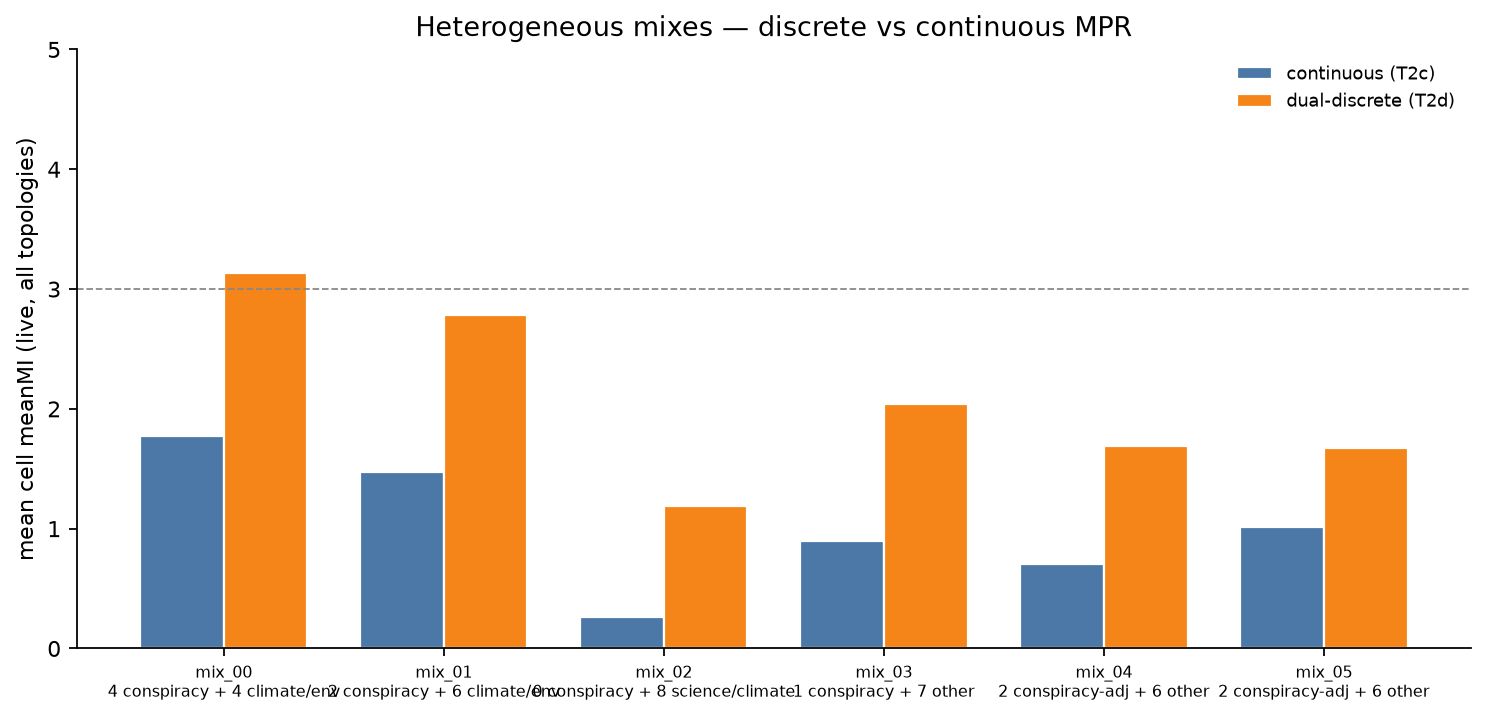
\includegraphics[width=\textwidth]{figures/fig04_mix_mpr_bars.png}
\caption{Heterogeneous mixes: live-cell mean \texttt{meanMI} collapsed across eight topologies, discrete versus continuous.
$N=1$, 48 cells per mix per mode before hatching.
Source: \texttt{fig04\_mix\_mpr\_bars.png}.}
\label{fig:mix}
\end{figure}

\begin{figure}[t]
\centering
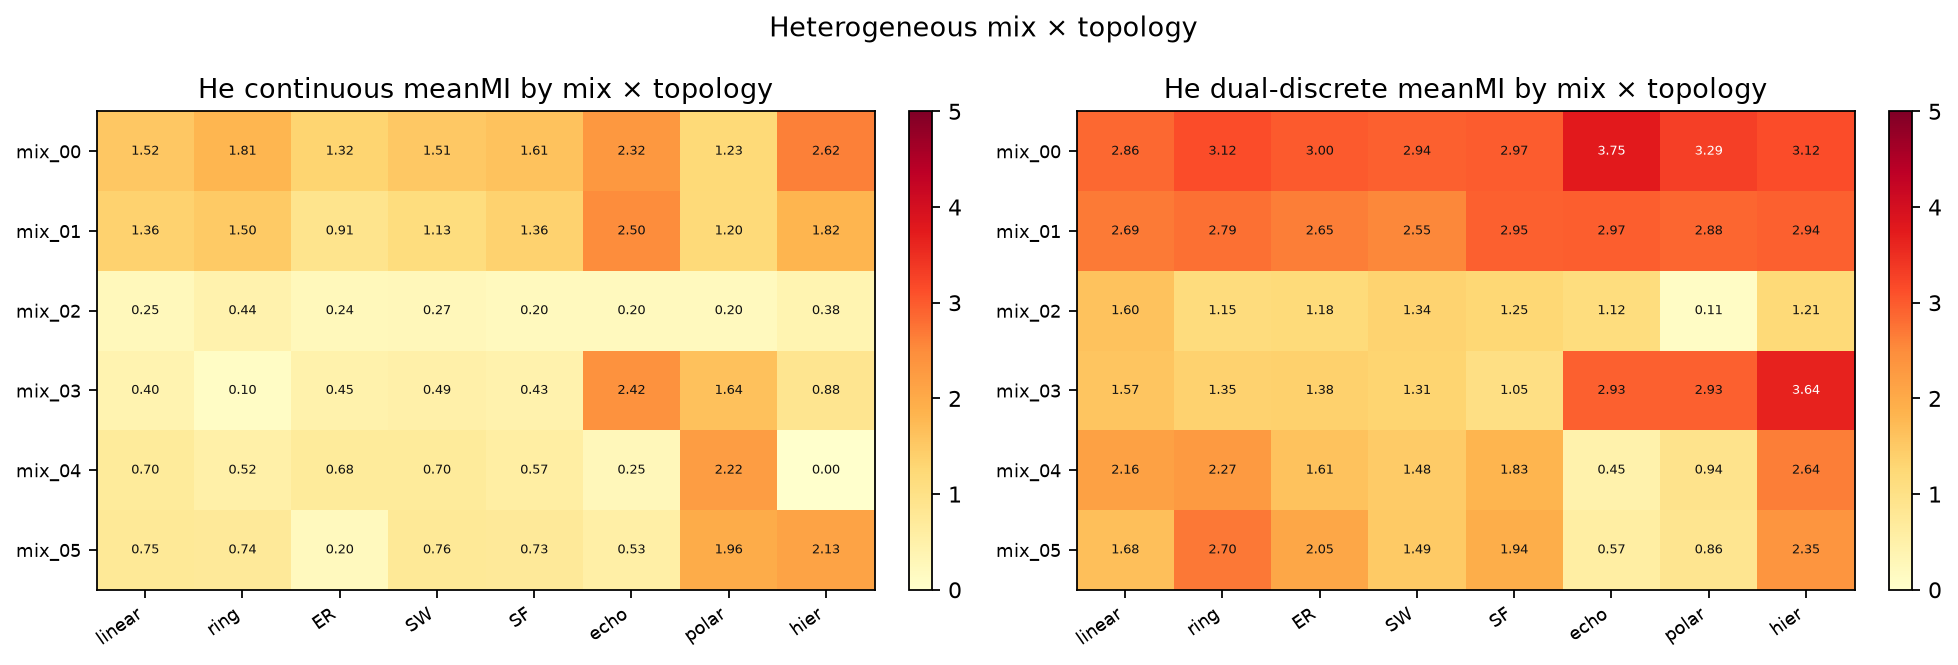
\includegraphics[width=\textwidth]{figures/fig07_mix_topology_heatmaps.png}
\caption{Heterogeneous mix $\times$ topology heatmaps of live-cell \texttt{meanMI}.
Left: continuous.
Right: dual-discrete.
$N=1$.
Source: \texttt{fig07\_mix\_topology\_heatmaps.png}.}
\label{fig:heatMT}
\end{figure}

\begin{table}[t]
\centering
\caption{Heterogeneous mixes collapsed across topologies.}
\label{tab:mix}
\begin{tabular}{llrrrr}
\toprule
Mix & Composition & Disc.\ \MPR{} & Cont.\ \MPR{} & \kstar{} dual & \kstar{} cont. \\
\midrule
mix\_00 & 4 conspiracy + 4 climate/env. & 3.1321 & 1.7712 & 57.5\% & 12.8\% \\
mix\_01 & 2 conspiracy + 6 climate/env. & 2.7795 & 1.4770 & 58.5\% & 9.8\% \\
mix\_02 & 0 conspiracy + 8 science/climate & 1.1882 & 0.2645 & 0.0\% & 0.0\% \\
mix\_03 & 1 conspiracy + 7 other & 2.0410 & 0.8945 & 33.3\% & 10.3\% \\
mix\_04 & 2 conspiracy-adj.\ + 6 other & 1.6896 & 0.7021 & 20.5\% & 5.3\% \\
mix\_05 & 2 conspiracy-adj.\ + 6 other & 1.6713 & 1.0134 & 23.3\% & 7.5\% \\
\bottomrule
\end{tabular}
\end{table}
